\documentclass[floatsintext,doc]{apa6}

\usepackage{amssymb,amsmath}
\usepackage{ifxetex,ifluatex}
\usepackage{fixltx2e} % provides \textsubscript
\ifnum 0\ifxetex 1\fi\ifluatex 1\fi=0 % if pdftex
  \usepackage[T1]{fontenc}
  \usepackage[utf8]{inputenc}
\else % if luatex or xelatex
  \ifxetex
    \usepackage{mathspec}
    \usepackage{xltxtra,xunicode}
  \else
    \usepackage{fontspec}
  \fi
  \defaultfontfeatures{Mapping=tex-text,Scale=MatchLowercase}
  \newcommand{\euro}{€}
\fi
% use upquote if available, for straight quotes in verbatim environments
\IfFileExists{upquote.sty}{\usepackage{upquote}}{}
% use microtype if available
\IfFileExists{microtype.sty}{\usepackage{microtype}}{}

% Table formatting
\usepackage{longtable, booktabs}
\usepackage{lscape}
% \usepackage[counterclockwise]{rotating}   % Landscape page setup for large tables
\usepackage{multirow}		% Table styling
\usepackage{tabularx}		% Control Column width
\usepackage[flushleft]{threeparttable}	% Allows for three part tables with a specified notes section
\usepackage{threeparttablex}            % Lets threeparttable work with longtable

% Create new environments so endfloat can handle them
% \newenvironment{ltable}
%   {\begin{landscape}\begin{center}\begin{threeparttable}}
%   {\end{threeparttable}\end{center}\end{landscape}}

\newenvironment{lltable}
  {\begin{landscape}\begin{center}\begin{ThreePartTable}}
  {\end{ThreePartTable}\end{center}\end{landscape}}




% The following enables adjusting longtable caption width to table width
% Solution found at http://golatex.de/longtable-mit-caption-so-breit-wie-die-tabelle-t15767.html
\makeatletter
\newcommand\LastLTentrywidth{1em}
\newlength\longtablewidth
\setlength{\longtablewidth}{1in}
\newcommand\getlongtablewidth{%
 \begingroup
  \ifcsname LT@\roman{LT@tables}\endcsname
  \global\longtablewidth=0pt
  \renewcommand\LT@entry[2]{\global\advance\longtablewidth by ##2\relax\gdef\LastLTentrywidth{##2}}%
  \@nameuse{LT@\roman{LT@tables}}%
  \fi
\endgroup}


  \usepackage{graphicx}
  \makeatletter
  \def\maxwidth{\ifdim\Gin@nat@width>\linewidth\linewidth\else\Gin@nat@width\fi}
  \def\maxheight{\ifdim\Gin@nat@height>\textheight\textheight\else\Gin@nat@height\fi}
  \makeatother
  % Scale images if necessary, so that they will not overflow the page
  % margins by default, and it is still possible to overwrite the defaults
  % using explicit options in \includegraphics[width, height, ...]{}
  \setkeys{Gin}{width=\maxwidth,height=\maxheight,keepaspectratio}
\ifxetex
  \usepackage[setpagesize=false, % page size defined by xetex
              unicode=false, % unicode breaks when used with xetex
              xetex]{hyperref}
\else
  \usepackage[unicode=true]{hyperref}
\fi
\hypersetup{breaklinks=true,
            pdfauthor={},
            pdftitle={Quantifying the benefits of using decision models with response time and accuracy data},
            colorlinks=true,
            citecolor=blue,
            urlcolor=blue,
            linkcolor=black,
            pdfborder={0 0 0}}
\urlstyle{same}  % don't use monospace font for urls

\setlength{\parindent}{0pt}
%\setlength{\parskip}{0pt plus 0pt minus 0pt}

\setlength{\emergencystretch}{3em}  % prevent overfull lines


% Manuscript styling
\captionsetup{font=singlespacing,justification=justified}
\usepackage{csquotes}
\usepackage{upgreek}



\usepackage{tikz} % Variable definition to generate author note

% fix for \tightlist problem in pandoc 1.14
\providecommand{\tightlist}{%
  \setlength{\itemsep}{0pt}\setlength{\parskip}{0pt}}

% Essential manuscript parts
  \title{Quantifying the benefits of using decision models with response time and
accuracy data}

  \shorttitle{Power gains of decision modelling}


  \author{Tom Stafford\textsuperscript{1}, Angelo Pirrone\textsuperscript{2}, Mike Croucher\textsuperscript{3}, \& Anna Krystalli\textsuperscript{4}}

  % \def\affdep{{"", "", "", ""}}%
  % \def\affcity{{"", "", "", ""}}%

  \affiliation{
    \vspace{0.5cm}
          \textsuperscript{1} Department of Psychology, University of Sheffield\\
          \textsuperscript{2} School of Psychological and Cognitive Sciences, Peking University\\
          \textsuperscript{3} Research Computing, University of Leeds\\
          \textsuperscript{4} Research Software Engineering, University of Sheffield  }

  \authornote{
    Address correspondance to
    \href{mailto:t.stafford@sheffield.ac.uk}{\nolinkurl{t.stafford@sheffield.ac.uk}}
    
    Correspondence concerning this article should be addressed to Tom
    Stafford, Department of Psychology, University of Sheffield, 1 Vicar
    Lane, Sheffield, S1 2LT, UK. E-mail:
    \href{mailto:t.stafford@sheffield.ac.uk}{\nolinkurl{t.stafford@sheffield.ac.uk}}
  }


  \abstract{Across diverse subfields experimentalists collect response time and
accuracy data. Inter-subject and inter-group speed-accuracy trade-offs
(SATOs) are a well-known possibility which are often inadequately
addressed. Many experiments focus on a single variable
(e.g.~psychophysics paradigms analysing accuracy alone), or involve a
suboptimal analytic correction (e.g.~dividing accuracy by response
time). Models of decision making, such as the drift diffusion model
(DDM), provide a principled account of the decision making process,
allowing the recovery of SATO-unconfounded decision parameters from
observed behavioural variables. For plausible parameters of a typical
between-groups experiment we simulate experimental data, for both real
and null group differences, and for both systematic and null SATOs, and
fit the DDM. This exercise allows us to make a number of concrete
recommendations for experimentalists: we show, in terms of reduction of
required sample size, how decision modelling allows more efficient data
collection for set statistical power; we confirm and depict the
non-linear speed-accuracy relation; we show how much more sensitive
accuracy is as a measure than response time.}
  \keywords{keywords \\

    \indent Word count: X
  }





\usepackage{amsthm}
\newtheorem{theorem}{Theorem}
\newtheorem{lemma}{Lemma}
\theoremstyle{definition}
\newtheorem{definition}{Definition}
\newtheorem{corollary}{Corollary}
\newtheorem{proposition}{Proposition}
\theoremstyle{definition}
\newtheorem{example}{Example}
\theoremstyle{definition}
\newtheorem{exercise}{Exercise}
\theoremstyle{remark}
\newtheorem*{remark}{Remark}
\newtheorem*{solution}{Solution}
\begin{document}

\maketitle

\setcounter{secnumdepth}{0}



\section{Abbreviations}\label{abbreviations}

DDM - Drift diffusion model

SATO - Speed-accuracy trade-off

\section{Introduction}\label{introduction}

\subsection{Speed accuracy trade-offs}\label{speed-accuracy-trade-offs}

Speed and accuracy of responding are fundamental measures of
performance, collected by behavioural scientists across diverse domains.
The two measures are related by the speed-accuracy trade-off (SATO). For
reviews of this topic see Wickelgren (1977); Heitz (2014).

The SATO is inextricably linked to the nature of decision making --- it
arises whenever we wish to respond as fast and as accurately possible
based on uncertain incoming information. More accurate responses require
more information, which takes longer to accumulate; faster responses
forgoe collecting additional information at the cost of higher error
rates. Importantly, because the SATO in unavoidable it is also necessary
that all decision-making processes are positioned with respect to the
trade-off. This does not need to be done deliberately or explicitly, but
any decision process can be characterised as adopting some trade-off
between speed and accuracy. For the tasks studied by psychologists, it
is important to recognise that there will be individual differences, as
well as task and group-related differences, in how participants position
themselves on the SATO.

Outside of researched focussed on SATOs explicitly, different practices
have been adopted to account for SATOs or potential SATOs in behavioural
data. One approach is to ignore either speed or accuracy. For example,
ignoring speed of response is common in psychophysics, whereas some
domains of cognitive psychology where high-accuracy is assumed, focus
only on response times (e.g. Stafford, Ingram, \& Gurney,
2011)\footnote{Note that we choose to cite work by the lead author here
  for illustration, rather than highlight any other researchers for
  their use of these suboptimal practices.}, sometimes after a cursory
check of error-rate data, or the failure of standard null-hypothesis
test to reveal signficiant differences in error-rates. Another approach
is to combine speed and accuracy. For example, in the domain of visual
search it is common to calculate `efficiency' scores by dividing search
time by search accuracy as a proportion (e.g. Yates \& Stafford, 2018).
Despite being widespread, there is evidence that this practice is
unlikely to add clarity to analysis (Bruyer \& Brysbaert, 2011). We also
note that the researchers who initially formulated the efficiency score
explictly counselled \emph{against} using it in the case of SATOs
(Townsend \& Ashby, 1983).

The efficiency score shares with other recent suggestions for accounting
for SATOs (Davidson \& Martin, 2013; Seli, Jonker, Cheyne, \& Smilek,
2013) the property that it assumes a linear relation between response
time and accuracy. While such approaches may be better than focussing on
a single behavioural variable, the assumption of linearity is at odds
with work which has explicitly characterised the SATO (Fitts, 1966;
Heitz, 2014; Wickelgren, 1977) and has shown distinct a distinctly
curvilinear relation between response time and accuracy. As such,
although linear correction methods may work for some portions of the
SATO, they are likely to be misleading, or at least fail to add clarity,
where accuracy and/or speed approaches upper or lower limits of those
variables.

\subsection{Context}\label{context}

The unprincipled combination of speed and accurary measures becomes an
urgent issue when considered in the context of widespread questions
surrounding the reliability of the literature in psychology. Established
results fail to replicate, or replicate with substantially reduced
effect sizes (Open Science Collaboration, 2015; Pashler \& Wagenmakers,
2012).

Low statistical power has been a persistent problem across many areas of
psychology and cognitive neuroscience (Button et al., 2013; Lovakov \&
Agadullina, 2017; Maxwell, 2004; Sedlmeier \& Gigerenzer, 1989; Stanley,
Carter, \& Doucouliagos, 2017; Szucs \& Ioannidis, 2017), including, but
not limited to, research areas which are bound by costly methods or
hard-to-reach populations (Bezeau \& Graves, 2001; J. Cohen, 1962;
Geuter, Qi, Welsh, Wager, \& Lindquist, 2018). This, combined with
factors such as analytic flexibility (Silberzahn et al., 2017; Simmons,
Nelson, \& Simonsohn, 2011) --- which can only be increased by a lack of
recognition of any optimal analysis method --- has led to a widespread
lack of faith in many published results (Ioannidis, 2005).

Statistical power is defined with respect to the variability and
availability of data, as well as the analysis proposed. For a set
experimental design, an obvious candidate for increasing stastical power
is to increase sample size, but this is not always easy. Each additonal
participant costs additonal time, money and resources. This is
especially true in the case of expensive methods, such as fMRI, or
special populations which may be hard to recruit. More sensitive
measures also increase statistical power: lower measurement error will
tend to reduce variability so that the same mean differences produce
larger observed effect sizes.

A motivation for the present work is to demonstrate the practical
utility, in terms of increased statistical power, of combining speed and
accuracy information in a principled manner. Such an innovation has the
appeal of making the most of data which is normally collected, even if
not analysed, whilst not requiring more participants (which is costly),
or more trials per participant (which also has costs in terms of
particpant fatigue which may be especially high for some popualations,
e.g.~children).

\subsection{Decision modelling}\label{decision-modelling}

Models of the decision making process provide the foundation for the
principled combination of speed and accuracy data, and thus afford
experimenters access to considerable statistical power gains.

Many models exist in which decision making is represented by the
accumulation of sensory evidence over time. When the accumulated
evidence surpasses some threshold (also called a boundary) then a
decision is triggered. The accuracy of the decision depends on which
accumator crosses which boudary, the speed is given by time this takes,
and thus such models can be used to fit speed and accuracy data within
the same framework.

A prominant instance of such accumulator models is the so called
drift-diffusion model developed by Roger Ratcliff (DDM Ratcliff, 1978;
Ratcliff \& Rouder, 1998). After a long and successful perdiod of
development and application on purely behavioural data, the DDM model
was at the centre of an important theoretical confluence.
Neurophysiologists found evidence for accumulation like processes in
neurons critical to sensory decision making (Gold \& Shadlen, 2001; P.
L. Smith \& Ratcliff, 2004), whilst theoreticians recognised that
accumulator models could be related to statistical methods of uncertain
information intregration (Bogacz, Brown, Moehlis, Holmes, \& Cohen,
2006; Gold \& Shadlen, 2002). Under certain parameterisations many
different decision models, all in the family of accumulator models, can
be shown to be equivalent to the DDM, and this in turn equivalent to a
statistical method which is optimal for making the fastest decision with
a given error rate (or the most accurate decision within a fixed time).

While debate continues around the exact specification of the decision
model which best reflects human decision making, there is a consensus
that the DDM captures many essential features of decision processesing
(but see Pirrone, Stafford, and Marshall (2014); Teodorescu, Moran, and
Usher (2016); Pirrone, Azab, Hayden, Stafford, and Marshall (2018)). As
you would expect, the DDM has also shown considerable success modelling
decision data across many different domains (Ratcliff \& McKoon, 2008).
In the sense that the DDM implements a statistically optimal algorithm
for accumulation for uncertain information, we would expect our neural
machinery to implement the same algorithm in the absence of other
constraints (Pirrone et al., 2014). The basic mechanism of the DDM is
illustrated in Figure \ref{fig:ddm}.

\begin{figure}

{\centering 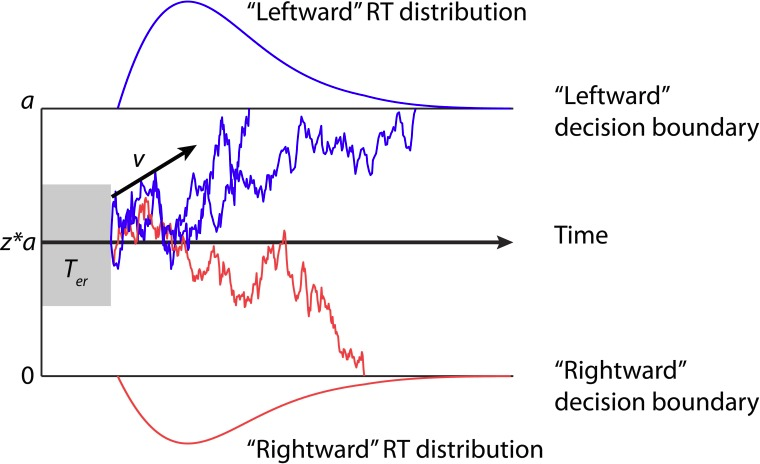
\includegraphics[width=0.6\linewidth]{figs/zhang_fig1} 

}

\caption{An illustration of the drift-diffusion model (DDM); taken from Zhang and Rowe, 2014. Here a decision between two choices, `leftward' and `rightward' is shown. Parameters labelled are $v$, the drift rate which reflects the rate of evidence accumulation; $\alpha$, the boundary seperation, which reflect response conservativeness; $z$, the starting point, which biases the response based on pre-stimulus expectations and $T_{er}$, non-decision time, a fixed delay which does not vary with stimulus information.}\label{fig:ddm}
\end{figure}

For our purposes, the value of these decision models is that they
provide a principled reconcilation of speed and accuracy data. Within
this framework these observed behavioural measures reflect the hidden
parameters of the decision model, most important of which (for our
purposes) are the drift rate and boundary seperation, which reflect the
strength of evidence accumulation (reflecting participant
sensivitiy/stimulus salience) and the decision boundary (reflecting the
conservativeness of the participant's decision criterion; higher
boundaries produce slower but more accurate responses).

By fitting the DDM we can deconfound the observed behavioural variables
--- speed and accuracy --- and recover the putative generating
parameters of the decision --- drift and boundary seperation. In
principle, this allows a more sensitive measure of participant
capability (reflected in the drift parameter). Drift is a more sensitive
measure because a) it is estimated using both speed \emph{and} accuracy
and b) it is isolated from the effect of different participant response
thresholds (which are reflected in the boundary parameter).

Previous authors have established the in-principle gains of this
approach. Within a psychophysics framework, Stone (2014) extended
Palmer, Huk, and Shadlen (2005)'s decision model to show that response
time and accuracy contain different, but possibly overlapping,
components of Shannon information about the perceived stimulus. If these
components do not overlap (as suggested by Stone, in preparation) then
combining response time and accuracy data should provide better
estimates of key parameters which govern the decision process than
relying on either response time or accuracy alone. Previous authors have
shown for specific paradigms and decisions that using decision models
confers benefits beyond relying on speed, accuracy or some sub-optimal
combination of the two, especially in the case of speed-accuracy
trade-offs (Park \& Starns, 2015; e.g. Zhang \& Rowe, 2014). Our purpose
here is not to make a theoretical innovation in decision modelling, but
to use established decision models to demonstrate and quantify the
benefits of decision modelling for experimentalists.

\section{Method}\label{method}

The broad approach is to consider a simple standard experimental design:
a between groups comparison each group contains a number of participants
who complete a number of decision trials, which provide both response
time and accuracy data. We simulate data for true and null differences
in drift (sensitivity) between the groups, as well as true and null
differences in boundary (SATO) between the groups. By varying the number
of simualated participants we generate a fixed number of `scenarios'
defined by true/null effects in sensitivty, true/null SATOs and
experimental sample size. For each scenario we inspect the behavioural
measures to see how senstive and specific they are to detecting true
group differences. We also fit the DDM and estimate the participant
drift parameters, similarly asking how sensitive and specific estimates
of drift are to true group differences in drift. An overview of the
method is provided in Figure \ref{fig:DDMprocess}.

\begin{figure}

{\centering 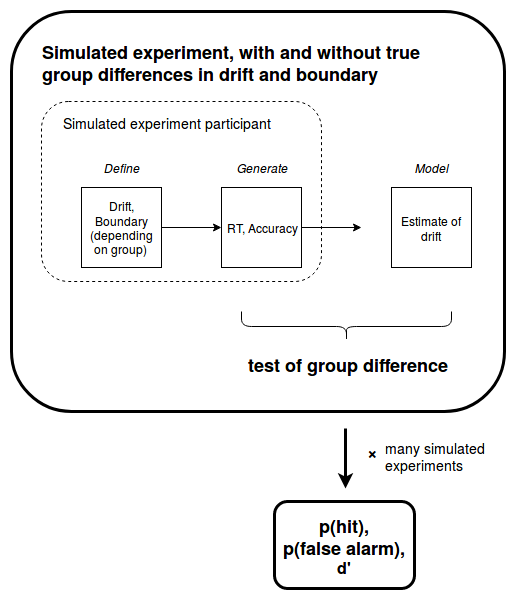
\includegraphics[width=0.75\linewidth]{figs/DDM_process_less} 

}

\caption{Overview of method}\label{fig:DDMprocess}
\end{figure}

\subsection{Decision modelling}\label{decision-modelling-1}

To generate simulated response data, and we use the Hieracrchical Drift
Diffusion Model (HDDM, Wiecki, Sofer, \& Frank, 2013). This toolbox can
also perform model fitting, which uses Bayesian estimation methods to
similtaneously fit individual decision parameters and the group
distributions from which they are drawn.

While the HDDM offers a principled and comprehensive model fitting
approach, it is computationally expensive. An alternative model fitting
method, the EZ-DDM (E.-J. Wagenmakers, Van Der Maas, \& Grasman, 2007)
offers a simple approximation, fitting a decision model with a smaller
number of parameters using an analytic method which is computationally
cheap. Furthermore, the EZ-DDM has been shown to match the full DDM for
a range of situations (Ravenzwaaij, Donkin, \& Vandekerckhove, 2017).

For the model fitting presented here (Figures \ref(fig:vanilla) -
\ref(fig:SATOdprime)), we use the EZ-DDM, although we have verified that
the results are qualitatively similar using the HDDM and the fast-ddm
(A. Voss \& Voss, 2007), a third model fitting framework, so we believe
that these results do not depend on the particular decision model
deployed from the broad class of accumulator models.

Obviously, where we wish to simulate many thousands of independent
experiments there are significant speed gains from parallelisation.
Parallalisation was done by Mike Croucher, and the code run on
University of Sheffield High Performance Computing cluser. A sense of
the value of parallelisation can be had by noting the the data shown in,
for example, Figure \ref(fig:SATOdprime) would have taken around 1
calander month to generate on a single high performance machine, using
the computationally `cheap' EZ-DDM method. Python code for running the
simulations, as well as the output data, figures and manuscript
preparation files, is here
\url{https://github.com/tomstafford/ddm_sims}.

\subsection{Analysis}\label{analysis}

Because we are not generating an analytic solution we cannot claim that
our findings are true for all situations. Our aim is merely to show that
for some reasonable choices of DDM parameters using decision modelling
is a superior approach to analysing response time or accuracy alone or
combining them in any suboptimal way.

To be able to make this claim of relevance of our simulations to typical
psychology experiments we need to be able to justify that our parameter
choice is plausible for a typical psychology experiment. In order to
establish this we pick parameters which generate response times of the
order of 1 second and accuracy of the order 90\%.\footnote{Note, for
  high accuracy values t-tests may not be appropriate (they are strictly
  not applicable to proportions anyway, but this may become a real issue
  for values very close to 1 or 0).}. Each participant contributes 40
decision (40 trials) to each experiment. Parameters for drift and
boundary seperation are defined for the group and individual participant
values for these parameters are drawn from the group parameters with
some level of variability (and, in the case of true effects, a mean
difference between the group values).

To illustrate this, we show in Figure \ref{fig:SATOdirect} a direct
visualation of the speed-accuracy trade-off, by taking the base
parameters we use in our simulated experiments and generating a single
particpant's average response time and accuracy, using 1000 different
boundary seperation values. This shows the effect of varying boundary
seperation alone, while all other decision parameters are stable.

\begin{figure}
\centering
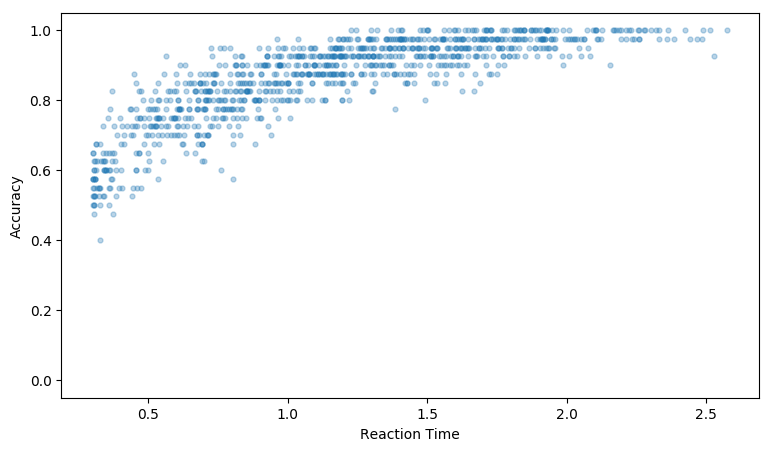
\includegraphics{figs/SATO-direct_scatter.png}
\caption{\label{fig:SATOdirect}Directly visualising the speed-accuracy
trade-off: average response time and accuracy from a single simulated
particpant with all decision parameters kept fixed except for boundary
seperation, which is drawn from a normal distibution (mean = 2, variance
= 1) (1000 simulated experiments, each of 40 trials}
\end{figure}

For each scenario we simulate a large number of experiments, with
participant parameters sampled each time from the defined distributions.
For each experiment, any difference between groups is gauged with a
standard two-sample t-test for the behavioural variables.

\subsubsection{Effect sizes}\label{effect-sizes}

The drift and boundary paramters for each each simulated participant are
drawn from declared group means, meaning that the true difference
between groups can be expressed in terms of Cohen's d effect size ---
the mean difference between the groups standardised by the within group
variability.

For the observed variables, response time and accuracy, the effect sizes
can only be observed, not declared, since these arise from the
interaction of the DDM parameters and the DDM model which generates
responses. The declared group difference in drift rate produces the
observed effect size in response time and accuracy (which differ from
each other), depending on both the level of noise in each simulated
experiment, and the experiment design - specifically on the number of
trials per participant.

Experiment designs which have a higher number of trials per participant
effectively sample the true drift rate more accurately, and so have
effect sizes for response time and accuracy which are closer to the
\enquote{true}, declared, effect size in drift rate.

This issue sheds light on why decision modelling is more effective than
analysing response time or accuracy alone (because it recovers the
generating parameter, drift, which is more sensitive to group
differences), and why there are differences in power between measuring
response time and accuracy (because these variables show different
observed effect sizes when generated by the same true different in drift
rates). Figure \ref{fig:effectsizes} shows how declared differences in
drift translate into observed effect sizes for response time and
accuracy.

\begin{figure}

{\centering 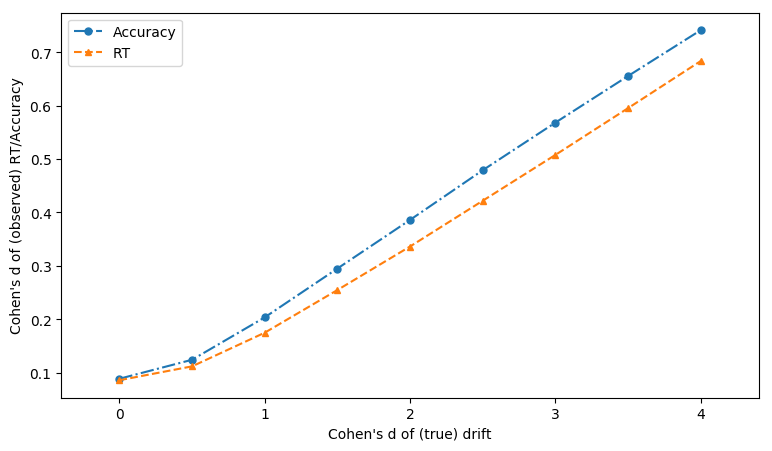
\includegraphics[width=0.68\linewidth]{figs/effectsizetranslation} 

}

\caption{How differences in drift convert to observed differences in response time and accuracy (40 trials per ppt)}\label{fig:effectsizes}
\end{figure}

\subsubsection{Hits (power) and False Alarms
(Alpha)}\label{hits-power-and-false-alarms-alpha}

Statistical power is the probability of your measure reporting a group
difference when there is a true group difference, analogous to the
\enquote{hit rate} in a signal detection paradigm. Conventional power
analysis assumes a standard false positive (\emph{alpha}) rate of 0.05.
For our simulations we can measure the actual false alarm rate, rather
than assume it remains at the intended 0.05 rate.

For analysing situations where only the drift differs between two groups
we would not expect any significant variations in false alarm rate.
However, when considering speed-accuracy trade-off changes between
groups (with or without drift rate differences as well) the situation is
different. This means that it is possible to get false positives in
tests of a difference in drifts between groups because of SATOs. Most
obviously, if a SATO means one group prioritises speed over accuracy,
analysis of response time alone will mimic an enhanced drift rate, but
analysis of accuracy alone will mimic degraded drift rate. Ideally the
DDM will be immune to any distortion of estimates of drift rates, but
that is what we have set out to demonstrate so we should not assume.

The consequence of this is that it makes sense to move calculating
measure sensitivity, accounting for both the false alarm rate, as well
as the hit rate. A principled way for combining false alarm and hit rate
into a single metric is d' (\enquote{d prime}), which gives an overall
sensitivity of the test, much as we would calculate the sensitivity
independent of bias for an observer in a psychophysics experiment
(Green, 1966)

\section{Results}\label{results}

The results shown here support our central claim that decision modelling
can have substantial benefits. To explore the interaction of power,
sample size, effect size and measure sensitivty we have prepared an
interactive visualisation which can be found here
\url{https://sheffield-university.shinyapps.io/decision_power/}

\subsection{Without Speed-Accuracy
Trade-offs}\label{without-speed-accuracy-trade-offs}

For an idea of the main implications, it is sufficient to plot a slice
of the data when the difference in drift is a Cohen's d of 2. Recall,
from Figure \ref{fig:effectsizes} above, that although this is a large
difference in terms of the generating parameter, drift, this translates
into small observed effect sizes in accuracy and response time.

Figure \ref{fig:vanilla}, right, shows how sample size and hit rate
interact for the different measures. The results will be depressingly
familiar to any experimentalist who has taken power analysis seriously
--- a sample size far larger than that conventionally recruited is
required to reach adequate power levels for small/medium group
differences.

\begin{figure}

{\centering 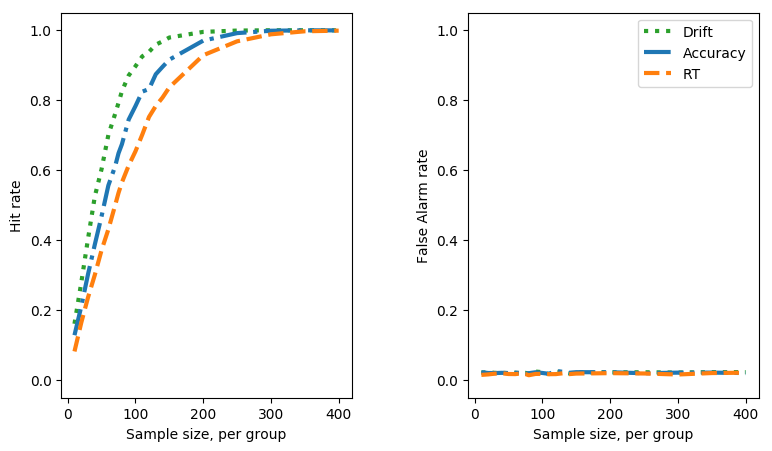
\includegraphics[width=0.68\linewidth]{figs/NOSATO_hit_and_FA} 

}

\caption{Simulated experiment sample size against hit rate and false alarm rate (for effect size of 2 vs 0, cohen'd d for drift parameter)}\label{fig:vanilla}
\end{figure}

From this figure we can read off the number of participants per group
required to reach the conventional 80\% power level (equivalent to hit
rate of 0.8, if we assume a constant false positive rate). For this part
of the parameter space, for this size of difference between groups in
drift, and no speed-accuracy trade-off, \textasciitilde{}140
participants are required to achieve 80\% power if the difference
between groups is tested on the speed of correct responses only. If the
difference between grouops is tested on the accuracy rate only then
\textasciitilde{}115 participants per group are required. If speed and
accuracy are combined using decision modelling, and difference between
groups tests on the recovered drift parameters then we estimate that
\textasciitilde{}55 participants per group are required for 80\% power.
An experimentalist who might have otherwise had to recruit 280 (or 230)
participants could therefore save herself (and her participants)
significant trouble, effort and cost by deploying decision modelling,
recruiting half that sample size and still enjoying an increase in
statistical power to detect group differences.

Figure \ref{fig:vanilla}, left, shows the false alarm rate. When the
difference in drifts is a Cohen's d of 0, i.e.~no true difference, the
t-tests on response time and accuracy both generate false alarm rates at
around the standard alpha level of \(0.05\)

Figure \ref{fig:vanilladprime} shows the measure sensitivity, d' for
each sample size. In effect, this reflects the hit rate (Figure
\ref{fig:vanillahits}) corrected for fluctuations in false alarm rate
(Figure \ref{fig:vanillaFAs}). This correction will be more important
when their are systemmatic variations in false poisitve rate due to
SATOs

\begin{figure}

{\centering 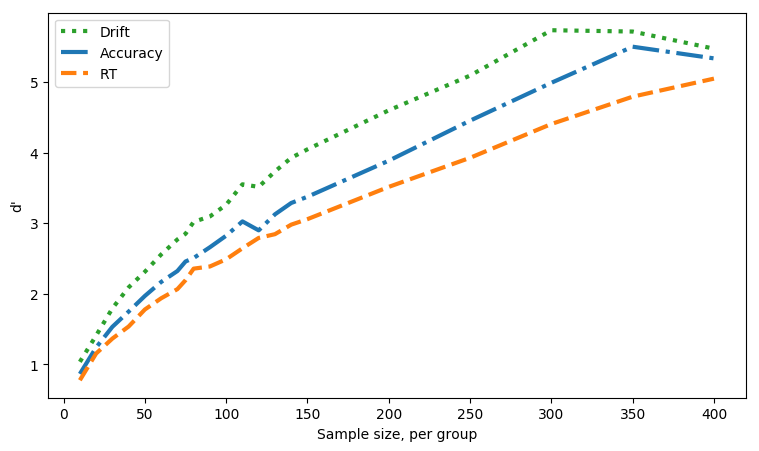
\includegraphics[width=0.68\linewidth]{figs/NOSATO_dprime} 

}

\caption{Simulated experiment sample size against d' (for effect size of 2 vs 0  cohen'd d for drift parameter)}\label{fig:vanilladprime}
\end{figure}

\subsection{With SATOs}\label{with-satos}

The superiority of parameter recovery via a decision model becomes even
more stark if there are systemmatic speed-accuracy trade-offs. To see
this, we re-run the simulatations above, but with a shift in the
boundary parameter before group A and group B, such that individuals
from group B have a lower boundary, and so tend to make faster but less
accurate decisions compared to group B. On top of this difference, we
simulate different sizes of superiority of drift rate of group B over
group A.

For the plots below, the drift rate difference is, as above, 0.1 (which,
given the interindividual variability translates into an effect size of
2). The boundary parameter difference is also 0.1, a between group
effect size 2.

Unlike when there are no SATOs, the response time measure is superior
for detecting a group difference than the drift measure, Figure
\ref{fig:SATO}, right.

\begin{figure}

{\centering 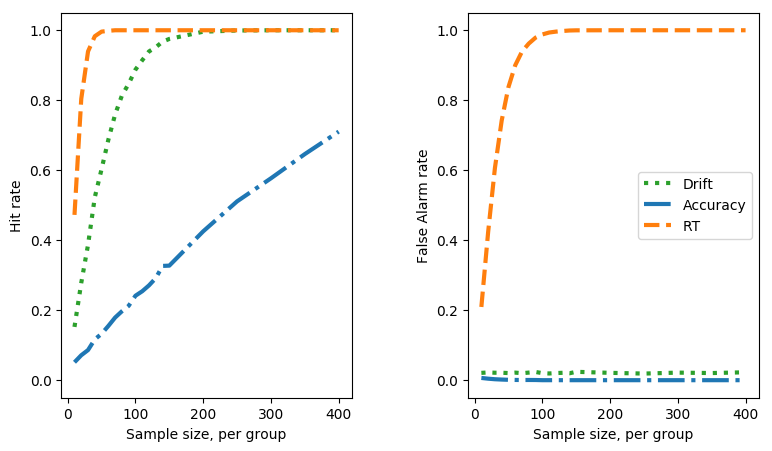
\includegraphics[width=0.68\linewidth]{figs/SATO_hit_and_FA} 

}

\caption{Simulated experiment sample size against hit rate and false alarm rate (for effect size of 2 vs 0, cohen'd d for drift parameter, and boundary parameter shifted 0.1 between groups)}\label{fig:SATO}
\end{figure}

This, however, is an artifact of the SATO. If the boundary shift had
been in the reverse direction then accuracy, not response time, would
appear the superior measure. Once we compare the false positive rate the
danger of using a single observed measure becomes clear, Figure
\ref{fig:SATO}, left.

When using the drift parameter as a measure the SATO between the groups
does not induce false alarms. The accuracy measure is insensitive so
also doesn't suffer (but would if the boundary shift was in the opposite
direction). The response time measure is catastrophically sensitive to
false alarms, approaching 100\% false alarm rate with larger samples.

Combining the hit rate and the false alarm rate to calculate d', and so
see measure sensitivity, Figure \ref{fig:SATOdprime}.

\begin{figure}

{\centering 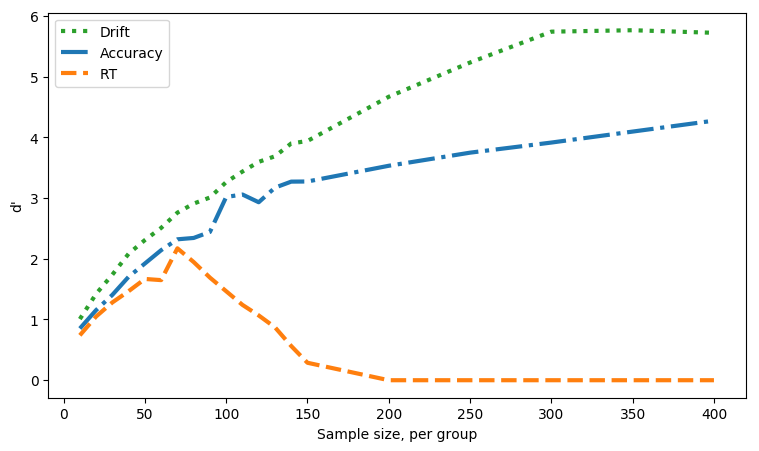
\includegraphics[width=0.68\linewidth]{figs/SATO_dprime} 

}

\caption{Simulated experiment sample size against d' (effect size = 2 cohen's d for drift parameter, 2 for boundary parameter)}\label{fig:SATOdprime}
\end{figure}

\section{Discussion}\label{discussion}

\subsection{Main conclusions}\label{main-conclusions}

We have shown the benefits of fitting response time and accuracy data
with standard decision models. Such decision models allow the estimation
of the generating parameters of simple perceptual decisions, such that
the participants sensitivity and response conservativeness are
deconfounded. This allows more powerful tests of between group
differences. In the presence of systemmatic shifts in the speed-accuracy
trade-off, this approach offers protection against false-positives or
false-negatives (in the case that SATOs disguise true differences in
sensitivty). We do not claim to make theoretical innovation in decision
modelling --- the work deploys widely used decision models `off the
shelf' and seeks to quantify the extrent of the benefit for
experimentalists of deploying decision modelling on their behavioural
data. The extent of the statistical power gain is considerable. The
exact benefit will vary according to the phenomenon and populations
investigated, as well as experimental design. For the example design and
parameter regime we showcase here the use of decision modelling allows
total sample size to be halved while still increasing statistical power.
To explore the relation of sample size and effect size to the
sensitivity of behavioural measures, and the decision modelling
measures, we provide an interactive data explorer here
\url{https://sheffield-university.shinyapps.io/decision_power/}

\subsection{Qualifications}\label{qualifications}

The results we showcase here and in the data explore hold only for the
parameter regime choosen. We have not analytically proved that parameter
recovery with the DDM will always provide a statistical power gain. We
have chosen a simple experimental design, with a plausible trial numbers
per participant and decision parameters which generate realistic values
for speed and accuracy of responses, but it is possible that for smaller
effects, at the boundaries of maximum or minimum speed or accuracy,
and/or with higher within and between participant noise, that decision
modelling may not have the benefits depicted here.

We have choose not to explore a within-participants design because the
issue of systemmatically different speed-accuracy trade-offs between
condtions seems, \emph{prima facie}, less likely. For between groups
designs we know of several prominent cases where systemmatic SATOs
confounded conclusions. For example Pirrone, Dickinson, Gomez, Stafford,
and Milne (2017) found that an apparent impairment of perceptual
judgement among Autism Spectrum Disorder (ASD) participants could be
attributed to a difference in their SATO. The ASD group responded more
conservatively, but decision modelling showed their had equivalent
senstivity to the non-ASD group. Ratcliff, Thapar, and McKoon (2006)
found an analogous result for young vs old participants on perceptual
discrimination and recognition memory tasks.

As well as occupying a particular point in the parameter space of
decision models, our results are also generated using a particular model
and model fitting approach (the EZ-DDM, E.-J. Wagenmakers et al., 2007),
although we have verfied that the same quantative pattern can be
produced by alternative approaches {[}@{]} For some parameterisations
several prominent decision models are equivalent (Bogacz et al., 2006).
A recent collaborative analysis project found that desite a large
diversity of fitting methods common inferences where across different
decision models (Dutilh et al., 2016). A reasonable conclusion from this
project was that in many circumstances the simple models should be
preferred (Lerche \& Voss, 2016). Ratcliff and Childers (2015) claims
that heirarchival bayesian methods of fitting, as we use here are best,
at least for individual difference investigations (although see Jones
and Dzhafarov (2014) who claim that many variants of the DDM cannot be
successfully distinguished by empirial measurement).

\subsection{Wider context}\label{wider-context}

As well as power gains, and protection against SATO confounds, decision
modelling has other benefits to offer the experimentalist. It allows
differences between participants or groups to be localised to particular
components of the decision process. Decision modelling, since it relies
on the distribution of responses rather than just the means, can also
reveal underlying differences when single variables (e.g.~response time)
are stable (White, Ratcliff, Vasey, \& McKoon, 2010)

There is a growing awareness of the limitations of studying only speed
or accuracy alone (Oppenheim, 2017). A recent meta-analysis confirms a
low correlation between speed and accuracy costs in psychological tasks
(Hedge, Powell, Bompas, Vivian-Griffiths, \& Sumner, in press).
Vandierendonck (2017) compares seven model-free transformations which
combine reaction time and accuracy, but finds none unambigiously
superior either to the others or to inspecting raw reaction time and
accuracy.

\subsection{Related work}\label{related-work}

A recent paper (Hedge, Powell, \& Sumner, 2018) used a comparable
simulation based approach reached a similar conclusion to ours --- that
model-free transformations of reaction time and accuracy, even if
hallowed by common usage, are outperformed by a model-based
transformation which assumes a sequential sampling model like the DDM.

White, Servant, and Logan (2018) also present a parameter recovery
account, but compare different variations of the sequential sampling
models which are designed to account for decisions under conflict. Their
focus is on comparing between different decision models rather than
model-free and model-based transformations of reaction time and accuracy

Baker et al. (2019) using the simulation method to address a question of
equal importance to experimentalist --- how does the number of trials
interact with sample size to affect statistical power. Like us they
present an interactive demonstration of their findings
\url{https://shiny.york.ac.uk/powercontours/}

\subsection{Getting started with decision
modelling}\label{getting-started-with-decision-modelling}

For those who wish to apply decision models to their data have a range
of tutorials available (A. Voss, Nagler, \& Lerche, 2013, Forstmann,
Ratcliff, and Wagenmakers (2016)), as well as statistical computing
packages which support model fitting (Wiecki et al., 2013,A. Voss and
Voss (2007))

\section{Acknowledgements}\label{acknowledgements}

Jim Stone for discussion of the project and reading the manuscript.
Feedback online and offline from the presentation of this work at the
International meeting of the Psychonomics Society in Amsterdam, May
2018.

\section*{References}\label{references}
\addcontentsline{toc}{section}{References}

\hypertarget{refs}{}
\hypertarget{ref-baker2019power}{}
Baker, D. H., Vilidaite, G., Lygo, F. A., Smith, A. K., Flack, T. R.,
Gouws, A. D., \& Andrews, T. J. (2019). Power contours: Optimising
sample size and precision in experimental psychology and human
neuroscience. \emph{arXiv Preprint arXiv:1902.06122}.

\hypertarget{ref-bezeau2001statistical}{}
Bezeau, S., \& Graves, R. (2001). Statistical power and effect sizes of
clinical neuropsychology research. \emph{Journal of Clinical and
Experimental Neuropsychology}, \emph{23}(3), 399--406.

\hypertarget{ref-bogacz2006physics}{}
Bogacz, R., Brown, E., Moehlis, J., Holmes, P., \& Cohen, J. D. (2006).
The physics of optimal decision making: A formal analysis of models of
performance in two-alternative forced-choice tasks. \emph{Psychological
Review}, \emph{113}(4), 700--765.

\hypertarget{ref-bruyer2011combining}{}
Bruyer, R., \& Brysbaert, M. (2011). Combining speed and accuracy in
cognitive psychology: Is the inverse efficiency score (ies) a better
dependent variable than the mean reaction time (rt) and the percentage
of errors (pe)? \emph{Psychologica Belgica}, \emph{51}(1), 5--13.

\hypertarget{ref-button2013power}{}
Button, K. S., Ioannidis, J. P., Mokrysz, C., Nosek, B. A., Flint, J.,
Robinson, E. S., \& Munafò, M. R. (2013). Power failure: Why small
sample size undermines the reliability of neuroscience. \emph{Nature
Reviews Neuroscience}, \emph{14}(5), 365--376.

\hypertarget{ref-cohen1962statistical}{}
Cohen, J. (1962). The statistical power of abnormal-social psychological
research: A review. \emph{The Journal of Abnormal and Social
Psychology}, \emph{65}(3), 145--153.

\hypertarget{ref-davidson2013modeling}{}
Davidson, D., \& Martin, A. E. (2013). Modeling accuracy as a function
of response time with the generalized linear mixed effects model.
\emph{Acta Psychologica}, \emph{144}(1), 83--96.

\hypertarget{ref-dutilh2016quality}{}
Dutilh, G., Annis, J., Brown, S. D., Cassey, P., Evans, N. J., Grasman,
R. P., \ldots{} others. (2016). The quality of response time data
inference: A blinded, collaborative assessment of the validity of
cognitive models. \emph{Psychonomic Bulletin \& Review}, 1--19.

\hypertarget{ref-fitts1966cognitive}{}
Fitts, P. M. (1966). Cognitive aspects of information processing: III.
set for speed versus accuracy. \emph{Journal of Experimental
Psychology}, \emph{71}(6), 849--57.

\hypertarget{ref-forstmann2016sequential}{}
Forstmann, B. U., Ratcliff, R., \& Wagenmakers, E.-J. (2016). Sequential
sampling models in cognitive neuroscience: Advantages, applications, and
extensions. \emph{Annual Review of Psychology}, \emph{67}, 641--666.

\hypertarget{ref-geuter2018effect}{}
Geuter, S., Qi, G., Welsh, R. C., Wager, T. D., \& Lindquist, M. A.
(2018). Effect size and power in fMRI group analysis. \emph{bioRxiv},
295048.

\hypertarget{ref-gold2001neural}{}
Gold, J. I., \& Shadlen, M. N. (2001). Neural computations that underlie
decisions about sensory stimuli. \emph{Trends in Cognitive Sciences},
\emph{5}(1), 10--16.

\hypertarget{ref-gold2002banburismus}{}
Gold, J. I., \& Shadlen, M. N. (2002). Banburismus and the brain:
Decoding the relationship between sensory stimuli, decisions, and
reward. \emph{Neuron}, \emph{36}(2), 299--308.

\hypertarget{ref-green1966signal}{}
Green, S. J., D.M. (1966). \emph{Signal detection theory and
psychophysics}. Wiley.

\hypertarget{ref-hedge2018mapping}{}
Hedge, C., Powell, G., \& Sumner, P. (2018). The mapping between
transformed reaction time costs and models of processing in aging and
cognition. \emph{Psychology and Aging}, \emph{33}(7), 1093.

\hypertarget{ref-hedgelow}{}
Hedge, C., Powell, G., Bompas, A., Vivian-Griffiths, S., \& Sumner, P.
(in press). Low and variable correlation between reaction time costs and
accuracy costs explained by accumulation models: Meta-analysis and
simulations. \emph{Psychological Bulletin}.

\hypertarget{ref-heitz2014speed}{}
Heitz, R. P. (2014). The speed-accuracy tradeoff: History, physiology,
methodology, and behavior. \emph{Frontiers in Neuroscience}, \emph{8},
150.

\hypertarget{ref-ioannidis2005most}{}
Ioannidis, J. P. (2005). Why most published research findings are false.
\emph{PLoS Medicine}, \emph{2}(8), e124.

\hypertarget{ref-jones2014unfalsifiability}{}
Jones, M., \& Dzhafarov, E. N. (2014). Unfalsifiability and mutual
translatability of major modeling schemes for choice reaction time.
\emph{Psychological Review}, \emph{121}(1), 1--32.

\hypertarget{ref-lerche2016model}{}
Lerche, V., \& Voss, A. (2016). Model complexity in diffusion modeling:
Benefits of making the model more parsimonious. \emph{Frontiers in
Psychology}, \emph{7}, 1324.

\hypertarget{ref-lovakov_agadullina_2017}{}
Lovakov, A., \& Agadullina, E. (2017, November). Empirically derived
guidelines for interpreting effect size in social psychology. PsyArXiv.
doi:\href{https://doi.org/10.17605/OSF.IO/2EPC4}{10.17605/OSF.IO/2EPC4}

\hypertarget{ref-maxwell2004persistence}{}
Maxwell, S. E. (2004). The persistence of underpowered studies in
psychological research: Causes, consequences, and remedies.
\emph{Psychological Methods}, \emph{9}(2), 147.

\hypertarget{ref-open2015estimating}{}
Open Science Collaboration. (2015). Estimating the reproducibility of
psychological science. \emph{Science}, \emph{349}(6251), aac4716.

\hypertarget{ref-oppenheim2017blind}{}
Oppenheim, G. M. (2017). A blind spot in correct naming latency
analyses. \emph{Cognitive Neuropsychology}, \emph{34}(1-2), 33--41.

\hypertarget{ref-palmer2005effect}{}
Palmer, J., Huk, A. C., \& Shadlen, M. N. (2005). The effect of stimulus
strength on the speed and accuracy of a perceptual decision.
\emph{Journal of Vision}, \emph{5}(5), 1--1.

\hypertarget{ref-park2015approximate}{}
Park, J., \& Starns, J. J. (2015). The approximate number system acuity
redefined: A diffusion model approach. \emph{Frontiers in Psychology},
\emph{6}, 1955.

\hypertarget{ref-pashler2012editors}{}
Pashler, H., \& Wagenmakers, E. (2012). Editors' introduction to the
special section on replicability in psychological science: A crisis of
confidence? \emph{Perspectives on Psychological Science}, \emph{7}(6),
528--530.

\hypertarget{ref-pirrone2018evidence}{}
Pirrone, A., Azab, H., Hayden, B. Y., Stafford, T., \& Marshall, J. A.
(2018). Evidence for the speed--value trade-off: Human and monkey
decision making is magnitude sensitive. \emph{Decision}, \emph{5}(2),
129--142.

\hypertarget{ref-pirrone2017understanding}{}
Pirrone, A., Dickinson, A., Gomez, R., Stafford, T., \& Milne, E.
(2017). Understanding perceptual judgment in autism spectrum disorder
using the drift diffusion model. \emph{Neuropsychology}, \emph{31}(2),
173--180.

\hypertarget{ref-pirrone2014natural}{}
Pirrone, A., Stafford, T., \& Marshall, J. A. (2014). When natural
selection should optimize speed-accuracy trade-offs. \emph{Frontiers in
Neuroscience}, \emph{8}, 73.

\hypertarget{ref-ratcliff1978theory}{}
Ratcliff, R. (1978). A theory of memory retrieval. \emph{Psychological
Review}, \emph{85}(2), 59--108.

\hypertarget{ref-ratcliff2015individual}{}
Ratcliff, R., \& Childers, R. (2015). Individual differences and fitting
methods for the two-choice diffusion model of decision making.
\emph{Decision}, \emph{2}(4), 237.

\hypertarget{ref-ratcliff2008diffusion}{}
Ratcliff, R., \& McKoon, G. (2008). The diffusion decision model: Theory
and data for two-choice decision tasks. \emph{Neural Computation},
\emph{20}(4), 873--922.

\hypertarget{ref-ratcliff1998modeling}{}
Ratcliff, R., \& Rouder, J. N. (1998). Modeling response times for
two-choice decisions. \emph{Psychological Science}, \emph{9}(5),
347--356.

\hypertarget{ref-ratcliff2006aging}{}
Ratcliff, R., Thapar, A., \& McKoon, G. (2006). Aging and individual
differences in rapid two-choice decisions. \emph{Psychonomic Bulletin \&
Review}, \emph{13}(4), 626--635.

\hypertarget{ref-van2017ez}{}
Ravenzwaaij, D. van, Donkin, C., \& Vandekerckhove, J. (2017). The ez
diffusion model provides a powerful test of simple empirical effects.
\emph{Psychonomic Bulletin \& Review}, \emph{24}(2), 547--556.

\hypertarget{ref-sedlmeier1989studies}{}
Sedlmeier, P., \& Gigerenzer, G. (1989). Do studies of statistical power
have an effect on the power of studies? \emph{Psychological Bulletin},
\emph{105}(2), 309--316.

\hypertarget{ref-seli2013enhancing}{}
Seli, P., Jonker, T. R., Cheyne, J. A., \& Smilek, D. (2013). Enhancing
sart validity by statistically controlling speed-accuracy trade-offs.
\emph{Frontiers in Psychology}, \emph{4}, 265.

\hypertarget{ref-silberzahn2017many}{}
Silberzahn, R., Uhlmann, E. L., Martin, D., Anselmi, P., Aust, F.,
Awtrey, E. C., \ldots{} others. (2017). Many analysts, one dataset:
Making transparent how variations in analytical choices affect results.

\hypertarget{ref-simmons2011false}{}
Simmons, J. P., Nelson, L. D., \& Simonsohn, U. (2011). False-positive
psychology: Undisclosed flexibility in data collection and analysis
allows presenting anything as significant. \emph{Psychological Science},
\emph{22}(11), 1359--1366.

\hypertarget{ref-smith2004psychology}{}
Smith, P. L., \& Ratcliff, R. (2004). Psychology and neurobiology of
simple decisions. \emph{Trends in Neurosciences}, \emph{27}(3),
161--168.

\hypertarget{ref-stafford2011pieron}{}
Stafford, T., Ingram, L., \& Gurney, K. N. (2011). Piéron's law holds
during stroop conflict: Insights into the architecture of decision
making. \emph{Cognitive Science}, \emph{35}(8), 1553--1566.

\hypertarget{ref-stanleymeta}{}
Stanley, T., Carter, E. C., \& Doucouliagos, H. (2017). \emph{What
meta-analyses reveal about the replicability of psychological research}.
Working paper, Deakin Laboratory for the Meta-Analysis of Research.
Retrieved from
\url{http://www.deakin.edu.au/__data/assets/pdf_file/0007/1198456/WhatMeta-AnalysesReveal_WP.pdf}

\hypertarget{ref-stone2014using}{}
Stone, J. V. (2014). Using reaction times and binary responses to
estimate psychophysical performance: An information theoretic analysis.
\emph{Frontiers in Neuroscience}, \emph{8}, 35.

\hypertarget{ref-szucs2017empirical}{}
Szucs, D., \& Ioannidis, J. P. (2017). Empirical assessment of published
effect sizes and power in the recent cognitive neuroscience and
psychology literature. \emph{PLoS Biology}, \emph{15}(3), e2000797.

\hypertarget{ref-teodorescu2016absolutely}{}
Teodorescu, A. R., Moran, R., \& Usher, M. (2016). Absolutely relative
or relatively absolute: Violations of value invariance in human decision
making. \emph{Psychonomic Bulletin \& Review}, \emph{23}(1), 22--38.

\hypertarget{ref-townsend1983stochastic}{}
Townsend, J. T., \& Ashby, F. G. (1983). \emph{Stochastic modeling of
elementary psychological processes}. CUP Archive.

\hypertarget{ref-vandierendonck2017comparison}{}
Vandierendonck, A. (2017). A comparison of methods to combine speed and
accuracy measures of performance: A rejoinder on the binning procedure.
\emph{Behavior Research Methods}, \emph{49}(2), 653--673.

\hypertarget{ref-voss2007fast}{}
Voss, A., \& Voss, J. (2007). Fast-dm: A free program for efficient
diffusion model analysis. \emph{Behavior Research Methods},
\emph{39}(4), 767--775.

\hypertarget{ref-voss2013diffusion}{}
Voss, A., Nagler, M., \& Lerche, V. (2013). Diffusion models in
experimental psychology: A practical introduction. \emph{Experimental
Psychology}, \emph{60}(6), 385.

\hypertarget{ref-wagenmakers2007ez}{}
Wagenmakers, E.-J., Van Der Maas, H. L., \& Grasman, R. P. (2007). An
ez-diffusion model for response time and accuracy. \emph{Psychonomic
Bulletin \& Review}, \emph{14}(1), 3--22.

\hypertarget{ref-white2010using}{}
White, C. N., Ratcliff, R., Vasey, M. W., \& McKoon, G. (2010). Using
diffusion models to understand clinical disorders. \emph{Journal of
Mathematical Psychology}, \emph{54}(1), 39--52.

\hypertarget{ref-white2018testing}{}
White, C. N., Servant, M., \& Logan, G. D. (2018). Testing the validity
of conflict drift-diffusion models for use in estimating cognitive
processes: A parameter-recovery study. \emph{Psychonomic Bulletin \&
Review}, \emph{25}(1), 286--301.

\hypertarget{ref-wickelgren1977speed}{}
Wickelgren, W. A. (1977). Speed-accuracy tradeoff and information
processing dynamics. \emph{Acta Psychologica}, \emph{41}(1), 67--85.

\hypertarget{ref-wiecki2013hddm}{}
Wiecki, T. V., Sofer, I., \& Frank, M. J. (2013). HDDM: Hierarchical
bayesian estimation of the drift-diffusion model in python.
\emph{Frontiers in Neuroinformatics}, \emph{7}, 14.

\hypertarget{ref-yates_stafford_2018}{}
Yates, D., \& Stafford, T. (2018, June). 'Cognitive strategy' in visual
search: How it works and when it generalises. PsyArXiv.
doi:\href{https://doi.org/10.17605/OSF.IO/5DUP8}{10.17605/OSF.IO/5DUP8}

\hypertarget{ref-zhang2014dissociable}{}
Zhang, J., \& Rowe, J. B. (2014). Dissociable mechanisms of
speed-accuracy tradeoff during visual perceptual learning are revealed
by a hierarchical drift-diffusion model. \emph{Frontiers in
Neuroscience}, \emph{8}, 69.






\end{document}
